\let\negmedspace\undefined
\let\negthickspace\undefined
\documentclass[journal]{article}
\usepackage[a5paper, margin=10mm, onecolumn]{geometry}
\usepackage{lmodern} % Ensure lmodern is loaded for pdflatex

\setlength{\headheight}{1cm} % Set the height of the header box
\setlength{\headsep}{0mm}     % Set the distance between the header box and the top of the text

\usepackage{gvv-book}
\usepackage{gvv}
\usepackage{cite}
\usepackage{textcomp}
\usepackage{amsmath,amssymb,amsfonts,amsthm}
\usepackage{algorithmic}
\usepackage{graphicx}
\graphicspath{{./figs/}}
\usepackage{textcomp}
\usepackage{xcolor}
\usepackage{txfonts}
\usepackage{listings}
\usepackage{enumitem}
\usepackage{mathtools}
\usepackage{gensymb}
\usepackage{comment}
\usepackage[breaklinks=true]{hyperref}
\usepackage{tkz-euclide} 
\usepackage{listings}
\usepackage{gvv}                                        
\def\inputGnumericTable{}                                 
\usepackage[latin1]{inputenc}                                
\usepackage{color}                                            
\usepackage{array}                                            
\usepackage{longtable}                                       
\usepackage{calc}                                             
\usepackage{multirow}                                         
\usepackage{hhline}                                           
\usepackage{ifthen}                                           
\usepackage{lscape}
\usepackage{circuitikz}
\tikzstyle{block} = [rectangle, draw, fill=blue!20, 
text width=4em, text centered, rounded corners, minimum height=3em]
\tikzstyle{sum} = [draw, fill=blue!10, circle, minimum size=1cm, node distance=1.5cm]
\tikzstyle{input} = [coordinate]
\tikzstyle{output} = [coordinate]


\begin{document}
	
	\bibliographystyle{IEEEtran}
	\vspace{3cm}
	
\title{4.11.24}
\author{EE25BTECH11047 - RAVULA SHASHANK REDDY}
\maketitle
\hrulefill
\bigskip 

\renewcommand{\thetable}{\theenumi}
\setlength{\intextsep}{10pt}

\textbf{Question:}\\  

Find the equation of the plane through the line of intersection of
\begin{align*}
\vec{r}^T (\vec{i} + 3\vec{j}) + 6 = 0,
\vec{r}^T (3\vec{i} - \vec{j} - 4\vec{k}) = 0
\end{align*}

which is at a unit distance from the origin.\\

\textbf{Solution:}

\begin{align}
\pi_1 &: 
 \vec{n}_1=\myvec{1\\3\\0}, \ c_1=-6, \\[1ex]
\pi_2 &: \vec{n}_2=\myvec{3\\-1\\-4}, \ c_2=0.
\end{align}

Family of planes:
\begin{align}
(\vec{n}_1+\lambda\vec{n}_2)^T\vec{x}&=c_1+\lambda c_2\\
\vec{n}^T\vec{x}  &= c
\end{align}

Distance condition:
\begin{align}
d&=\frac{|\vec{n}^T\vec{x}-c|}{||\vec{n}||}\\
\vec{x}&=\vec{0}
\end{align}
\begin{align}
\frac{|c_1+\lambda c_2|}{\|\vec{n}_1+\lambda\vec{n}_2\|}=1
\quad\Longrightarrow\quad
(c_1+\lambda c_2)^2=(\vec{n}_1+\lambda\vec{n}_2)^T(\vec{n}_1+\lambda\vec{n}_2)
\end{align}
\begin{align}
36&=\vec{n}_1^T\vec{n}_1+2\lambda\vec{n}_1^T\vec{n}_2+\lambda^2\vec{n}_2^T\vec{n}_2\\
\vec{n}_1^T\vec{n}_1&=1^2+3^2=10,\\
\vec{n}_1^T\vec{n}_2&=1.3+3.(-1)+0.(-4)=0,\\
\vec{n}_2^T\vec{n}_2&=3^2+(-1)^2+(-4)^2=26
\end{align}

Hence:
\begin{align}
36=10+26\lambda^2
\quad\Longrightarrow\quad
26\lambda^2=26
\quad\Longrightarrow\quad
\lambda=\pm1
\end{align}

For $\lambda=1$:
\begin{align}
\myvec{-\tfrac{2}{3}&-\tfrac{1}{3}&\tfrac{2}{3}}\vec{x}=1
\end{align}

For $\lambda=-1$:
\begin{align}
\myvec{\tfrac{1}{3}&-\,\tfrac{2}{3}&-\,\tfrac{2}{3}}\vec{x}=1
\end{align}
\newpage
\begin{figure}
    \centering
    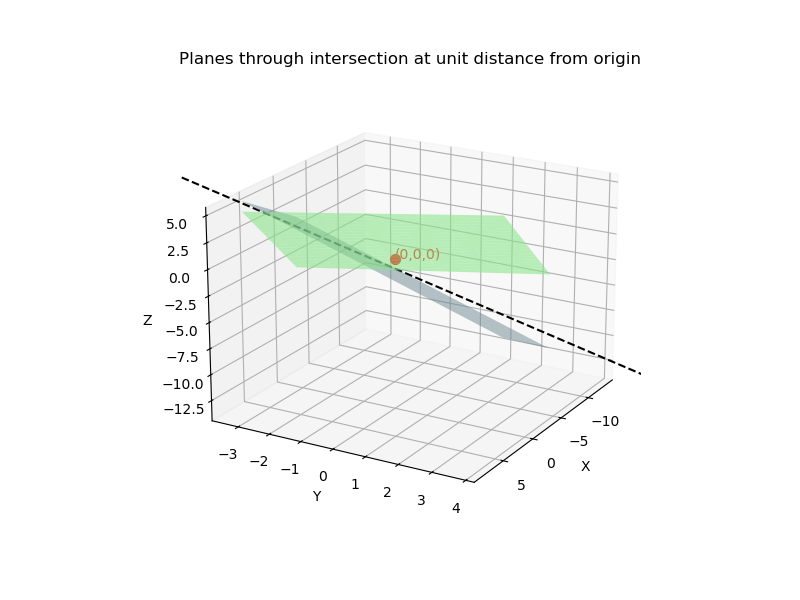
\includegraphics[width=1.0\linewidth]{figs/Figure_1.png}
    \caption{}
    \label{fig:placeholder}
\end{figure}
\end{document}
